\documentclass[10pt, a4]{seminar}
\usepackage{german}
\usepackage{graphicx}
\usepackage{semhelv}      % Helvetica Schriftart fuer Seminar
% \slideframe{none}   % keine Rahmen fuer die Slides
\landscapeonly      % Landscape definition
\newpagestyle{NamedFrame}
{}
{
 \tiny{Clemens Lode, Seminar ,,Biologische Prinzipien in der Informatik'' 2006\hfil
 \tiny{\SlideTopicEntry}\hfil
 \theslide }
}
\usepackage{sem-a4}

\setlength{\pdfpagewidth}{6in}
\setlength{\pdfpageheight}{4in}

\begin{document}
\renewcommand{\SlideTopicEntry}{}          % Topic fuer den Footer
\renewcommand{\SlideTitleEntry}{Vortrag Humorale Immunantwort}  % Titel in den Header
\pagestyle{NamedFrame}

\begin{slide}
\pagestyle{EmptyFrame}
\begin{center}
{\bf\LARGE Humorale Immunantwort}\\
{\bf Menschliches Immunsystem und Anwendungen in der Informatik}\\
\vspace{1cm}
\end{center}
\end{slide}

\slideframe{UnderlinedFrame}


\begin{slide}
\myslideheading{Inhalt des Vortrags}
\begin{itemize}
\item Grunds"atzlicher Ablauf der Immunantwort
\item Immunisierung
\item Effektive Erkennung von Fremdk"orper
\item Humorale Immunantwort
\item Klonale Selektion
\item Selbst-Fremd-Erkennung
\item Anwendungen der Informatik
\end{itemize}

\vfill
\end{slide}


\begin{slide}
\begin{figure}[h]
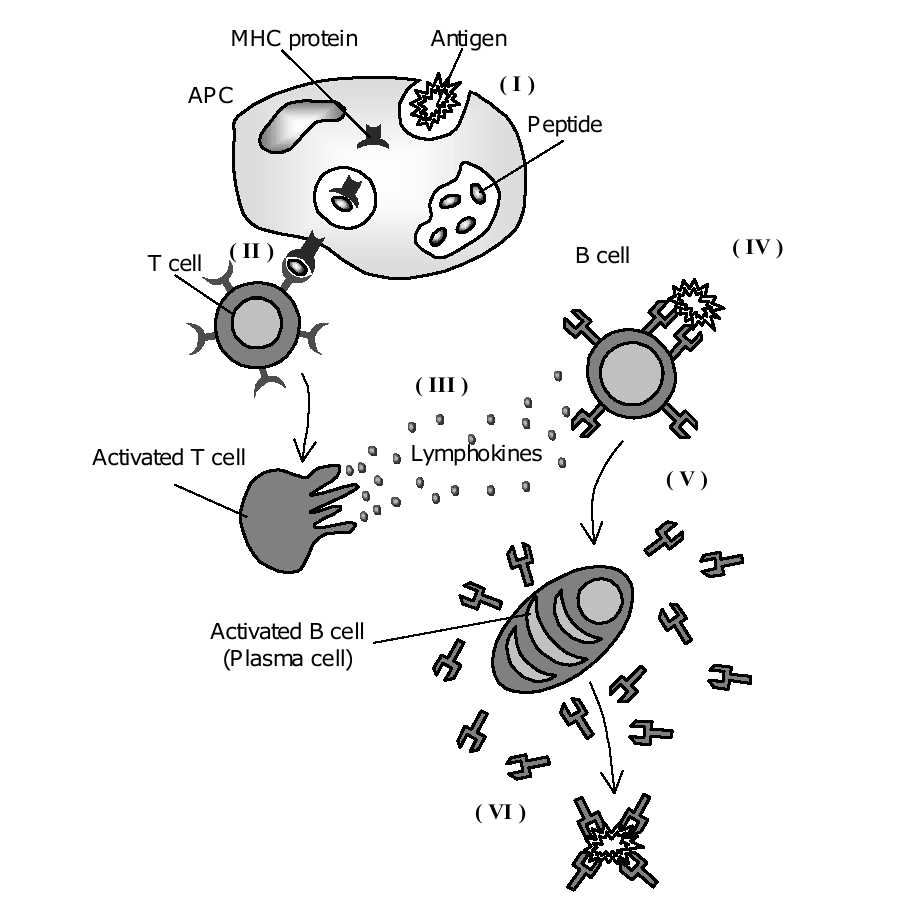
\includegraphics[scale=0.2]{immunablauf.png}
\caption{Ablauf einer Immunantwort}
\end{figure}
\vfill
\end{slide}

\begin{slide}
\myslideheading{Grunds"atzlicher Ablauf einer Immunantwort}
\begin{itemize}
\item Makrophagen durchqueren den K"orper und nehmen Antigene von Fremdk"orpern auf (I)
\item Aus Antigenen werden MHC-Molek"ule gebildet und auf der Oberfl"ache pr"asentiert (II)
\item Eine T-Zelle mit passendem Rezeptor kann an der Makrophage andocken und wird dadurch aktiviert
\item Die aktivierte Zelle sch"uttet Lymphokine aus, die B-Zellen aktivieren (III)
\item Die B-Zellen docken an Antigene bzw. antigenpr"asentierende Fremdk"orper (IV)
\item Die aktivierte B-Zelle teilt sich in antik"orperproduzierende Plasmazellen und in langlebige Ged"achtniszellen als Schutz f"ur sp"atere Infektionen (V)
\item Die Antik"orper binden sich an die Antigene und markieren so die damit verbundenen Fremdk"orper (VI)
\end{itemize}

\vfill
\end{slide}

\begin{slide}
\begin{figure}[h]
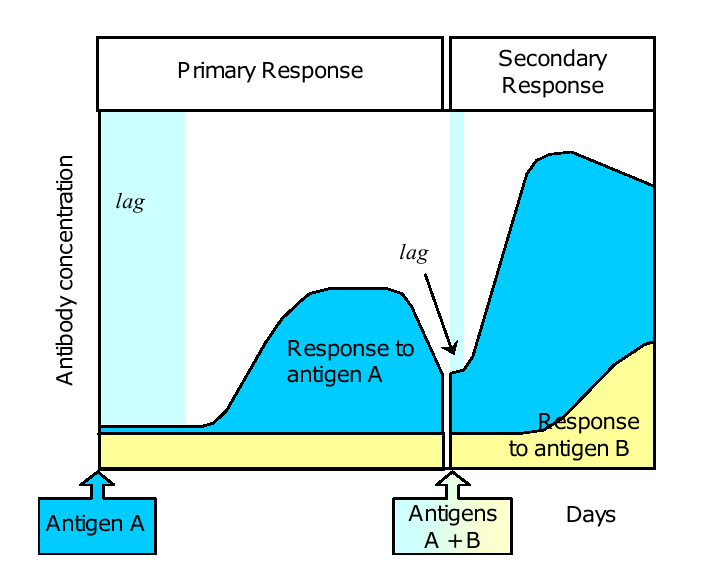
\includegraphics[scale=0.3]{immunsekundaer.png}
\caption{Prim"are und sekund"are Immunantwort}
\end{figure}
\vfill
\end{slide}

\begin{slide}
\myslideheading{Immunantwort}
\begin{itemize}
\item Anlegung von Ged"achtniszellen nach erstem Kontakt
\item Sehr schnelle Antwort durch Ged"achtniszellen bei zweitem Kontakt
\item Aktivimpfung als ungef"ahrlichere M"oglichkeit der Immunisierung
\item Passivimpfung mit Antik"orpern
\item Alleine durch Passivimpfung werden keine Ged"achtniszellen angelegt
\end{itemize}
\vfill
\end{slide}


\begin{slide}
\myslideheading{Ablauf Immunreaktion}
\begin{itemize}
\item B-Zellen sind f"ur Antik"orperproduktion zustaendig
\item Pr"asentieren Antigene auf der Oberfl"ache
\item Sicherheitsmechanismus "uber T-Zellen, keine Aktivierung von B-Zellen ohne aktivierte T-Zellen
\item Aktivierung von T-Zellen "uber Makrophagen
\item Aktivierung von B-Zellen erst wenn sowohl B-Zellen als auch T-Zellen das Antigen erkannt haben
\item Teilen der B-Zelle in antik"orperproduzierende Plasmazellen und langlebige Ged"achtniszellen
\item Jeder Antik"orper erkennt eine Reihe "ahnlicher dreidimensionaler Proteinstrukturen
\item Verankerung mit den Antigenen, Markierung des Fremdk"orpers zur Vernichtung
\end{itemize}
\vfill
\end{slide}


\begin{slide}

\begin{figure}[h]
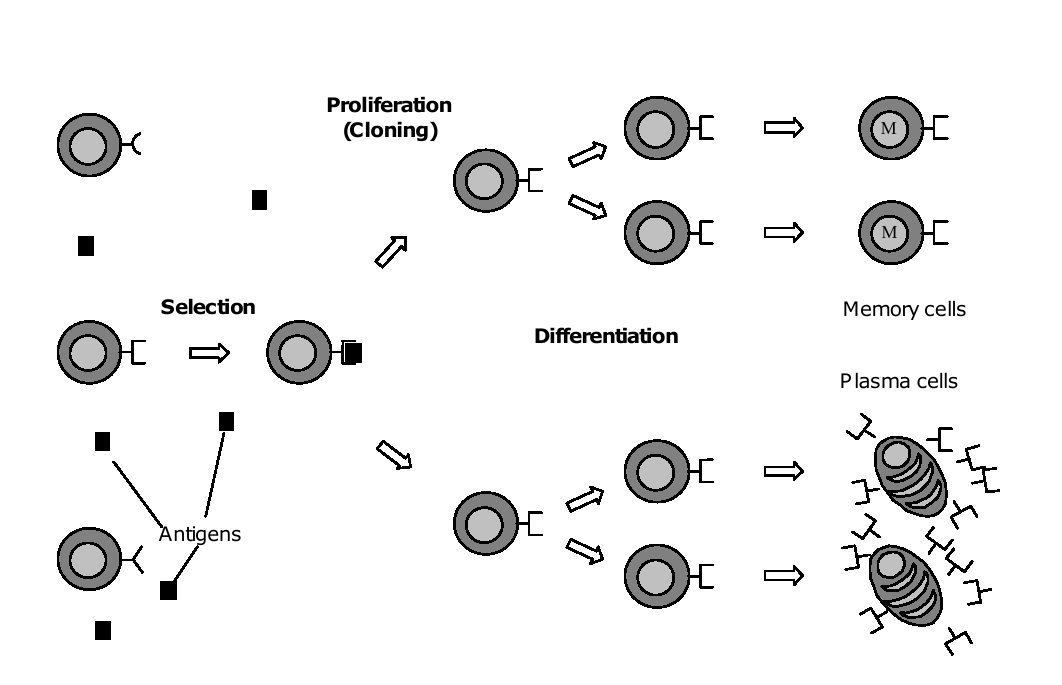
\includegraphics[scale=0.25]{immuncloning.png}
\caption{Klonale Selektion, B-Zellen mit hoher Antigenaffinit"at werden ausgew"ahlt}
\end{figure}
\vfill
\end{slide}

\begin{slide}
\myslideheading{Klonale Selektion}
F. McFarlane Burnet: ,,Einzelne Lymphozyten mit bestimmter Antigenspezifit"at sind in geringer Zahl vorhanden (pr"aexistieren) und werden aktiviert und vermehrt wenn das Antigen auftritt.''\\
\begin{itemize}
\item Zellklonung ist mit Mutation und Rekombination der Gene verbunden
\item Jede Lymphocyte hat individuelle Antigenspezifit"at
\item Erkennung praktisch aller Fremdk"orper
\item Entscheidender Punkt: Zeit bis ein Fremdk"orper erkannt wurde
\item Menschlicher K"orper: \(10^{6}\) Proteine, Immunsystem muss aber \(10^{16}\) Proteine bzw. Strukturen erkennen
\item Durch Kombination k"onnen etwa \(10^{15}\) Arten von Rezeptoren gebildet werden
\item Tats"achlich nur etwa \(10^{8}\) bis \(10^{12}\) zu einem Zeitpunkt
\item Ausgleich "uber ungenaue Bindung und andauernde Neubildung
\end{itemize}
\vfill
\end{slide}


\begin{slide}
\myslideheading{Selbst-Fremd-Erkennung}
\begin{itemize}
\item K"orpereigene Zellen haben typische Oberfl"achenstrukturen (eindeutiges Merkmal: MHC)
\item T-Zellen die diese erkennen werden im Thymus durch selektive Deletion entfernt (ca. 95\%)
\item B-Zellen dezentral, keine selektive Deletion, ben"otigen T-Zellen um aktiv zu werden
\item Fehler in der selektiven Deletion f"uhren zu Autoimmunkrankheiten
\item Beispiel Bluttransfusion: Blutzellen besitzen Antigenkombinationen 0 (keine Antigene), A, B und AB
\item Blutgruppe 0 kann an jeden spenden, aber nur von 0 empfangen
\item Blutgruppe AB kann von jedem empfangen, aber nur an AB spenden
\item Blutgruppe A (B) kann nur von 0 und A (B) empfangen und an AB und A (B) spenden
\item Wichtig: Immunit"at existiert bereits ohne Kontakt mit Blut, Bakterien haben "ahnliche Oberfl"achenstrukturen
\item Sonderfall Rhesus-Faktor, Passivimpfung mit Anti-Rh-Antik"orpern
\end{itemize}
\vfill
\end{slide}

\begin{slide}
\myslideheading{Umsetzung in der Informatik}
\begin{itemize}
\item Umsetzung am Computer erlaubt einige Vereinfachungen (z.B. auch ohne Parallelisierung m"oglich)
\item Darstellung der Antik"orper und Antigene als Bitstrings
\item 0 passt auf 1 und 0, 1 passt nur auf 0, ,,r"aumliche Erhebung''
\item Zuf"allige Erstellung der Bitstrings, selektive Deletion
\item Definition der Antigenaffinit"at, Fitness (Zahl passender Bits minus Zahl nicht passender Bits)
\item Beispiel: 10111 : 01101 \(\Rightarrow\) Fitness 1, 10111 : 01001 \(\Rightarrow\) Fitness 3
\end{itemize}
\vfill
\end{slide}


\begin{slide}
\myslideheading{Immunalgorithmus}
\ \\
{\raggedright
\\
Erstelle eine Anzahl n zuf"alliger Antik"orper ( n \(\ll\) \(2^{bitstringlaenge}\) )\\
Schleife Beginn\\
\ \ \ Entferne Antik"orper die k"orpereigene Antigene erkennen\\
\ \ \ Pr"ufe die Fitness der Antik"orper bez"uglich der sich momentan im System befindlichen Antigene\\
\ \ \ W"ahle die Antik"orper mit der h"ochsten Fitness\\
\ \ \ L"osche die Antik"orper mit der geringsten Fitness\\
\ \ \ Klone die besten Antik"orper um wieder n Antik"orper im System zu haben\\
\ \ \ Mutiere die neuen Antik"orper\\
Schleife Ende\\
}
\vfill
\end{slide}

\begin{slide}
\myslideheading{Beispiel}
K"orperfremde Antigene: 1011, 1001, 0001\\
K"orpereigene Antigene: 0010, 1011\\
n = 4\\
\ \\
Antik"orper a1, a2, a3, a4: 0000, 1000, 0100, 1011\\
Fitness a1: 3 + 2 + 1 = 6\\
Fitness a2: 1 + 0 + 2 = 3\\
Fitness a3: - wird entfernt, erkennt k"orpereigenes Antigen\\
Fitness a4: -3 + -1 + 1 = -3\\
\ \\
a1 und a2 werden ausgew"ahlt und zuf"allig an einer Stelle mutiert:\\
neue Antik"orper: 0010, 0001, 1100, 1001\\
Fitness a1: 1 + 3 + 2 = 6\\
Fitness a2: 1 + 0 + -1 = 0\\
Fitness a3: 2 + 1 + 3 = 6\\
Fitness a4: -1 + -2 + 0 = -3\\
\ \\
a1 und a3 werden ausgew"ahlt und zuf"allig an einer Stelle mutiert:\\
neue Antik"orper: 0010, 0001, 1100, 1001\\
Fitness a1: 1 + 3 + 2 = 6\\
Fitness a2: 1 + 0 + -1 = 0\\
Fitness a3: 2 + 1 + 3 = 6\\
Fitness a4: -1 + -2 + 0 = -3\\
\vfill
\end{slide}

\begin{slide}
\myslideheading{Anwendungen in der Informatik}
\begin{itemize}
\item Immunalgorithmus im Kern nichts anderes als eine Spezialanwendung des evolution"aren Algorithmus
\item M"ogliche Anwendungen vielf"altig, z.B. Robotersteuerung, Optimierung, Sicherheit, Verteilte Agenten, Neuronale Netzwerke, Bild- und Mustererkennung
\item Virendetektion: Suchen von Virensignaturen, Auslegung von ,,decoy programs'' im Speicher, Warnen anderer, m"oglicherweise infizierter Computer
\begin{figure}[h]
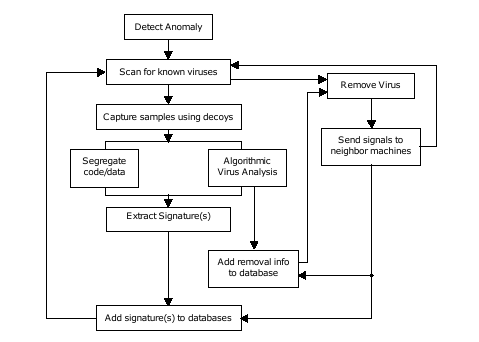
\includegraphics[scale=0.5]{immunvirus.png}
\caption{Virendetektion im Computer}
\end{figure}
\item Netzwerkueberwachung: Kategorisierung nach Merkmalen des Netzflusses, stichprobenartige Entnahme von Datenpaketen, Kodierung als Bitstrings
\end{itemize}
\vfill
\end{slide}


\begin{slide}
\myslideheading{Weiterf"uhrende Literatur}
\begin{itemize}
\item Leandro Nunes de Castro, Fernando Jose Von Zuben 1999: Artificial Immune Systems: Part I - Basic Theory and Applications, ftp://ftp.dca.fee.unicamp.br/pub/docs/vonzuben/tr\underline\ dca/trdca0199.pdf
\item Leandro Nunes de Castro, Fernando Jose Von Zuben 2000: Artificial Immune Systems: Part II - A Survey of Applications, ftp://ftp.dca.fee.unicamp.br/pub/docs/vonzuben/tr\underline\ dca/trdca0200.pdf
\item Steven A. Hofmeyr 1997: An Overview of the Immune System, http://www.cs.unm.edu/~immsec/html-imm/immune-system.html
\item Oder einfach: google ,,k"unstliches Immunsystem''
\end{itemize}
\vfill
\end{slide}

\end{document}
